\documentclass[]{fairmeta}
% Option "twocolumn" available, but please prioritize single-column

\usepackage{graphicx}
\usepackage{amsmath}
\usepackage{amssymb}
\usepackage{booktabs}
\usepackage{adjustbox}
\usepackage{multirow}
\usepackage{arydshln}
\usepackage{colortbl}
\usepackage{overpic}
\usepackage{amsthm}

\usepackage{amsfonts}       % blackboard math symbols
\usepackage{nicefrac}       % compact symbols for 1/2, etc.
\usepackage{microtype}      % microtypography

\usepackage{scalerel}
\newcommand{\sicong}[1]{{\color{blue}#1}}
\usepackage{makecell}

\usepackage{algorithm}
\usepackage{algorithmic}
\usepackage{enumitem}

% define ours package
\usepackage{nicefrac}
\usepackage{multirow}
\usepackage{booktabs}
\usepackage{float}
\usepackage{wrapfig}
\usepackage{bbding}
\usepackage{pifont}
\usepackage{color, colortbl}

\newcommand{\tabincell}[2]{\begin{tabular}{@{}#1@{}}#2\end{tabular}} % \tabincell{c}{
% \newcommand{\hr}[1]{\textcolor{blue}{#1}}
\newcommand{\hr}[1]{\textcolor{black}{#1}}
\definecolor{gray}{gray}{0.9}
\newcommand{\ssymbol}[1]{^{\@fnsymbol{#1}}}
\def\R{\mathbb{R}}
\newcommand{\Lleft}{\left(}
\newcommand{\Rright}{\right)}

\newtheorem{theorem}{Theorem}
\newtheorem{definition}{Definition}
\newtheorem{lemma}{Lemma}
\newtheorem{proposition}{Proposition}

\newcommand{\modelname}{LongVU}

\title{Efficient Track Anything}

\author[1,\dagger]{Yunyang Xiong}
\author[1,2]{Chong Zhou}
\author[1]{Xiaoyu Xiang}
\author[1]{Lemeng Wu}
\author[1]{Chenchen Zhu}
\author[1]{Zechun Liu}
\author[1]{Saksham Suri}
\author[1]{Balakrishnan Varadarajan}
\author[1]{Ramya Akula}
\author[1]{Forrest Iandola}
\author[1,\dagger]{Raghuraman Krishnamoorthi}
\author[1,\dagger]{Bilge Soran}
\author[1,\dagger]{Vikas Chandra}

\affiliation[1]{Meta AI}
\affiliation[2]{Nanyang Technological University}

\contribution[\dagger]{Project lead}

\abstract{Segment Anything Model 2 (SAM 2) has emerged as a powerful tool for video object segmentation and tracking anything. Key components of SAM 2 that drive the impressive video object segmentation performance include a large multistage image encoder for frame feature extraction and a memory mechanism that stores memory contexts from past frames to help current frame segmentation. The high computation complexity of multistage image encoder and memory module has limited its applications in real-world tasks, e.g., video object segmentation on mobile devices. To address this limitation, we propose EfficientTAMs, lightweight track anything models that produce high-quality results with low latency and model size. Our idea is based on revisiting the plain, nonhierarchical Vision Transformer (ViT) as an image encoder for video object segmentation, and introducing an efficient memory module, which reduces the complexity for both frame feature extraction and memory computation for current frame segmentation. We take vanilla lightweight ViTs and efficient memory module to build EfficientTAMs, and train the models on SA-1B and SA-V datasets for video object segmentation and track anything tasks. We evaluate on multiple video segmentation benchmarks including semi-supervised VOS and promptable video segmentation, and find that our proposed EfficientTAM with vanilla ViT perform comparably to SAM 2 model (HieraB+SAM 2) with $\sim$2x speedup on A100 and $\sim$2.4x  parameter reduction. On segment anything image tasks, our EfficientTAMs also perform favorably over original SAM with $\sim$20x  speedup on A100 and $\sim$20x  parameter reduction. On mobile devices such as iPhone 15 Pro Max, our EfficientTAMs can run at $\sim$10 FPS for performing video object segmentation with reasonable quality, highlighting the capability of small models for on-device video object segmentation applications.}

% \date{\today}
\correspondence{\email{yunyang@meta.com}}

\metadata[Project]{\url{https://yformer.github.io/efficient-track-anything/}}

\begin{document}

\maketitle

\vspace{-10pt}
\section{Introduction}
\label{sec:intro}
Autoregressive (AR) and diffusion models are two powerful paradigms for data distribution modeling. AR models, also known as the next token prediction approach, dominate language modeling and are considered central to the success of large language models (LLMs)~\cite{gpt1,gpt2,gpt3,llama1,llama2,llama3}. On the other hand, diffusion models~\cite{ddpm,dit,adm,edm}, or score-based generative models~\cite{songscore,lipman2023flow}, have emerged as the leading approach for visual generation, driving unprecedented progress in the era of visual content generation~\cite{sora,rombach2022high,li2023scaling}. 

\begin{figure}[t]
    \centering
    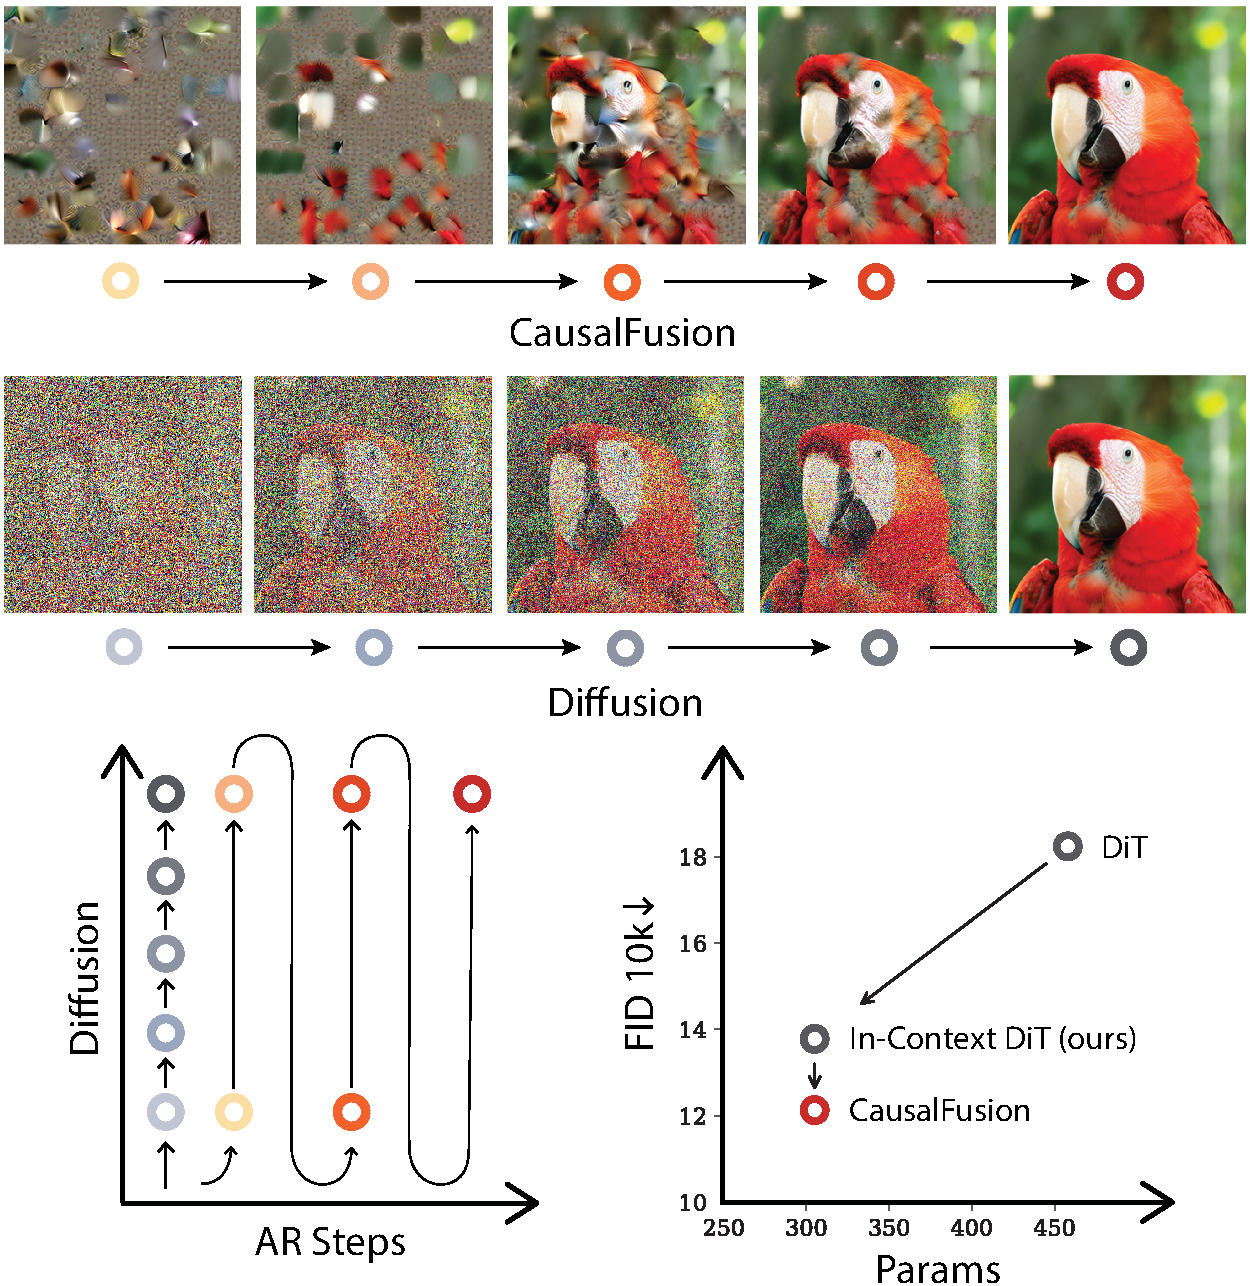
\includegraphics[width=1.0\textwidth,height=1.0\textwidth]{figs/casualfusion-teaser-v6.pdf} 
    \vspace*{-6mm}
    \caption{
    \textbf{Illustration of Dual-Factorization}. The arrow line indicates CausalFusion's generation path, moving from one state to the next by jointly generating along the sequential and noise-level dimension at each step. 
    Compared to DiT, our In-context DiT substantially improves results with fewer parameters. CausalFusion further enhances performance without changing the architecture or parameter count. Results were trained on IN1K for 240 epochs. CausalFusion adopts arbitrary AR steps for image generation, but each step only diffuses partial tokens, resulting in similar (or slightly lower) computational complexity.
    \vspace{-10pt}
    }
    \label{fig:dual-factorization}
\end{figure}


\begin{figure*}[t]
  \centering
  \begin{subfigure}{1.0\linewidth}
    \centering
    \includegraphics[width=\linewidth]{figs/figure2.pdf}
    \caption{Samples generated by CausalFusion-XL/2, ImageNet 512$\times$512, 800 epoch, DDPM 250 steps, CFG=4.0}
  \end{subfigure}
  \begin{subfigure}{1.0\linewidth}
    \centering
    \includegraphics[width=\linewidth]{figs/edit.pdf}
    \caption{\textbf{Zero-shot image editing} results generated by CausalFusion-XL/2, ImageNet 512$\times$512, 800 epoch. We first generate the original image (those on the left), then mask out its centre region, top-half, or bottom-half, and regenerate the image with new class conditions. Details are discussed in Sec \ref{sec:system}.}
  \end{subfigure}
  \caption{\textbf{Visualization results}. All samples are generated by models trained only on \textbf{ImageNet-1K class-conditional generation} task, demonstrating CausalFusion's zero-shot image manipulation ability. See more visualization results in Appendix~\ref{appendix:secD}.
  \vspace{-12pt}
  }
  \vspace{-6pt}
  \label{fig:vis1}
\end{figure*}

The intrinsic distinction between AR and diffusion models lies in their approach to data distribution factorization. AR models treat data as an ordered sequence, factorizing it along the sequential axis, where the probability of each token is conditioned on all preceding tokens. This factorization enables the AR paradigm to generalize effectively and efficiently across arbitrary number of tokens, making it well-suited for long-sequence reasoning and in-context generation. In contrast, diffusion models factorize data along the noise-level axis, where the tokens at each step are a refined (denoised) version of themselves from the previous step. As a result, the diffusion paradigm is generalizable to arbitrary number of data refinement steps, enabling iterative quality improvement with scaled inference compute. While AR and diffusion models each excel within their respective domains, their distinct factorization approaches reveal complementary potential. Although recent studies~\cite{transfusion,monoformer,dart} have attempted to integrate AR and diffusion within a single model, they typically treat these paradigms as separate modes, missing the potential benefits of jointly exploring them within a 2-D factorization plane.

To this end, we introduce \textbf{CausalFusion}, a flexible framework that integrates both sequential and noise-level data factorization to unify their advantages. The degree of factorization along these two axes—namely, the AR step and diffusion step—is adjustable, enabling {CausalFusion} to revert seamlessly to the traditional AR or diffusion paradigms at either extreme. To enhance its generality, CausalFusion is designed to predict \textit{any} number of tokens at \textit{any} AR step, with \textit{any} pre-defined sequence order and \textit{any} level of inference compute, thereby minimizing the inductive biases presented in existing generative models. As shown in Figure~\ref{fig:dual-factorization}, this approach provides a broad spectrum between the AR and diffusion paradigms, allowing smooth interpolation within two endpoints during both training and inference. 
Specifically, we explore CausalFusion in image generation and multimodal generation scenarios, where we observe that the level of training difficulties significantly influences the overall effectiveness of CausalFusion.

\textbf{Difficulties of generative tasks in CausalFusion:} Both AR and diffusion paradigms present unique challenges based on difficulties of their specific generative stages. In diffusion models, the effectiveness of training depends heavily on proper loss weighting across noise levels~\cite{ddpm,minsnr}, as higher noise levels are more difficult and usually provide more valuable signals than lower noise levels. Similarly, AR models are susceptible to error accumulation~\cite{bengio2015scheduled} as early-stage predictions are made with limited visible context, making them more error-prone. Optimizing CausalFusion thus requires balancing across these varying task difficulties to optimize training signal impact and ensure sufficient exploration across the entire factorization plane.

In this paper, we formally examine the difficulties of generative tasks within CausalFusion. We show that, in addition to the noise levels in diffusion and the amount of visible context in AR, the total number of AR steps, which controls the interpolation between AR and diffusion, also plays a critical role in shaping training difficulties. Driven by these factors, we develop a scalable and versatile model based on the CausalFusion framework. Starting from the DiT architecture~\cite{dit}, we gradually convert it into a decoder-only transformer compatible with existing AR models like GPT~\cite{gpt1,gpt2,gpt3} and LLaMA~\cite{llama1,llama2,llama3}. We provide insights on how to appropriately choose the number of AR steps during the training of CausalFusion models, and further introduce loss weighing along both the diffusion and AR axis to balance the impact of different generative stages. As shown in Figure~\ref{fig:dual-factorization} and ~\ref{fig:vis1}, our model achieves state-of-the-art performance on the ImageNet class-conditional generation benchmark, significantly outperforming DiT~\cite{dit} and enabling zero-shot image manipulations due to its AR nature. When pretraining on both text-to-image and image-to-text tasks, our model surpasses forced-fusion frameworks such as TransFusion~\cite{transfusion}, demonstrating the versatility of our CausalFusion framework.


We highlight our main contribution below:
\begin{itemize}
\item  We propose CausalFusion as the AR counterpart to DiT, achieving state-of-the-art results and enabling the unlimited token generation for in-context reasoning.
\item  We systematically study CausalFusion on the dual-factorization plane and identify key factors that improve the effectiveness of CausalFusion models.
\item  Compared with recent studies~\cite{transfusion}, CausalFusion enables a smooth, cohesive integration with language modeling for cross-modal generation and reasoning.
\end{itemize} 

% \begin{figure}[t]
%   \begin{minipage}{0.49\textwidth}
%      \centering
%     \includegraphics[width=1.0\textwidth]{fig/MLMF.png}
%     \caption{Multi-Layer Motion Fusion.}
%     \label{fig: frameselector_abalation}
    
%   \end{minipage}
%   \hfill
%    \begin{minipage}{0.48\textwidth}
%     \centering
%     \includegraphics[width=0.8\textwidth]{fig/SMPL.jpg}
%     \caption{Prametric Shape Alignment.}
%     \label{fig:Visualizedselected_frames}
%   \end{minipage}
% \vspace{-3mm}
% \end{figure}


\section{Related Work}
\label{sec:related_work}

\textbf{Diffusion Models for Image Generation.}
Diffusion-based models~\cite{balaji2022ediffi,huang2023composer,nichol2021glide,ramesh2022hierarchical,rombach2022high,saharia2022photorealistic} have rapidly emerged as a fundamental component in the domain of text-to-image generation, renowned for their capacity to yield highly promising generative outcomes. 
To address the considerable computational requirements inherent in diffusion models, the Latent Diffusion Model, as proposed in~\cite{rombach2022high} introduces a technique for denoising within the latent space.
This method not only enhances the computational efficiency of these models but also preserves their ability to generate high-fidelity images.
Moreover, in the endeavor to enhance control over visual generation, recent studies such as ControlNet~\cite{zhang2023adding}, T2I-Adapter~\cite{mou2023t2i}, and IP-Adapter~\cite{ye2023ip} have delved into the incorporation of supplementary encoder layers.
These layers facilitate the assimilation of control signals encompassing aspects such as pose, depth, and edge information, and even permit the utilization of images in conjunction with textual prompts.
This progression signifies a significant advancement towards more controlled and precise image generation, facilitating the creation of images characterized by not only superior quality but also enriched contextual accuracy and detail.


\textbf{Diffusion Models for Human Image Animation.}
The task of animating human images, a significant endeavor within the domain of video generation, aims to seamlessly create videos from one or multiple static images~\cite{chan2019everybody,ren2020deep,siarohin2019first,siarohin2021motion,yu2023bidirectionally,zhang2022exploring,zhao2022thin,yoon2021pose, sarkar2021neural, hu2023sherf, albahar2023humansgd, cao2023dreamavatar, prokudin2021smplpix, fu2022styleganhuman, jiang2023humangen}.
The recent advancements of diffusion models in the text-to-image domain have sparked interest in exploring their utility for animating human images.
PIDM~\cite{bhunia2023person} introduces a texture diffusion module that is specifically crafted to align the texture patterns of the source and target images closely, thereby enhancing the realism of the resultant animated output.
DreamPose~\cite{karras2023dreampose} capitalizes on the capabilities of the pre-trained Stable Diffusion model by incorporating both CLIP~\cite{radford2021learning} and VAE~\cite{kingma2013auto} for image encoding. 
It integrates these embeddings with an adapter. 
Similarly, DisCo~\cite{wang2023disco} innovatively segregates the control of pose and background using dual independent ControlNets~\cite{zhang2023adding}, providing finer control over the animation process. 
Animate Anyone~\cite{hu2023animate} utilizes a UNet-based ReferenceNet to extract features from reference images.
It includes pose information via a lightweight pose guider. Expanding on the principles introduced by AnimateDiff~\cite{guo2023animatediff}, Animate Anyone integrates a temporal layer into the denoising UNet to enhance temporal coherence.
MagicAnimate~\cite{xu2023magicanimate} follows a similar approach but employs a ControlNet tailored for DensePose \cite{guler2018dense} inputs instead of the more commonly used OpenPose~\cite{cao2017realtime} keypoints to provide more precise pose guidance.
This paper primarily builds upon esteemed diffusion-based methodologies and advances the optimization of appearance alignment and motion guidance mechanisms. 
This is achieved by introducing a 3D parametric model for geometric reconstruction of the reference image and motion modeling of the source video sequence.


\textbf{Pose Guidance in Human Image Animation.}
DWpose\cite{yang2023effective} stands out as an enhanced alternative to OpenPose\cite{cao2017realtime}, offering more accurate and expressive skeletons. 
This improvement has proven beneficial for diffusion models in generating higher quality images, with its adoption as a condition signal in various works\cite{feng2023dreamoving,hu2023animate}.
The work presented in DensePose~\cite{Guler2018DensePose} aims to establish dense correspondences between an RGB image and a surface-based representation.
The SMPL~\cite{SMPL:2015} model is a 3D model renowned for its realistic depiction of human bodies through skinning and blend shapes.
Its widespread adoption spans fields like human reconstruction\cite{he2021arch,alldieck2018video} and interaction with environments\cite{hassan2021populating,ma2020learning}. 
It also serves as essential ground truth for neural networks in pose and shape analysis\cite{lu2023dposer,mu2023actorsnerf}.
In this paper, we consider SMPL, the 3D parametric model, to reconstruct the poses as well as the shapes from the source video, and obtain more complete condition for appearance alignment and pose guidance.

\begin{figure}[t]
  \centering
  \includegraphics[width=0.95\linewidth]{fig/framework.jpg}
  \caption{The overview of our proposed approach. Given an input human image and a reference video depicting a motion sequence. We obtain the pose sequence corresponding to the reference image through Parametric Shape Alignment as 3D motion guidance. MLMF is employed to encode multi-layer 3D-related motion information. Referencenet and Temporal-attention ensure identity consistency and temporal coherence, respectively.}
  \vspace{-6mm}
  \label{fig:network}
\end{figure}
\section{Method}
%%%%%%%%% Figure: Overall framework
\begin{figure*}[t]
  \centering
   \includegraphics[width=0.85\linewidth]{figures/PoolFormer_overall_architecture.pdf}
   \vspace{-4mm}
   \caption{\textbf{(a) The overall framework of \modelname{}.} Similar to \cite{resnet, pvt, swin}, \modelname{} adopts hierarchical architecture with 4 stages. For a model with L \modelname{} blocks, stage [1, 2, 3, 4] have [L/6, L/6, L/2, L/6] blocks, respectively. The feature dimension $D_i$ of stage $i$ is shown in the figure. \textbf{(b) The architecture of \modelname{} block.} Compared with Transformer block, it replaces attention with extremely simple non-parametric operator, pooling, to conduct only basic token mixing.}
   \label{fig:overall_architecture}
\end{figure*}


%%%%%%%%% Algorithm: Pooling
\begin{algorithm}[t]
\caption{Pooling for PoolFormer, PyTorch-like Code}
\label{alg:code}
\definecolor{codeblue}{rgb}{0.25,0.5,0.5}
\definecolor{codekw}{rgb}{0.85, 0.18, 0.50}
\lstset{
  backgroundcolor=\color{white},
  basicstyle=\fontsize{7.5pt}{7.5pt}\ttfamily\selectfont,
  columns=fullflexible,
  breaklines=true,
  captionpos=b,
  commentstyle=\fontsize{7.5pt}{7.5pt}\color{codeblue},
  keywordstyle=\fontsize{7.5pt}{7.5pt}\color{codekw},
}
\begin{lstlisting}[language=python]
import torch.nn as nn

class Pooling(nn.Module):
    def __init__(self, pool_size=3):
        super().__init__()
        self.pool = nn.AvgPool2d(
            pool_size, stride=1, 
            padding=pool_size//2, 
            count_include_pad=False,
        )
    def forward(self, x):
        """
        [B, C, H, W] = x.shape
        Subtraction of the input itself is added 
        since the block already has a 
        residual connection.
        """
        return self.pool(x) - x
\end{lstlisting}
\end{algorithm}

\subsection{MetaFormer}
We present the core concept ``MetaFormer" for this work at first. As shown in Figure \ref{fig:first_figure}, abstracted from Transformers \cite{transformer}, 
MetaFormer is a general architecture where the token mixer is not specified while the other components are kept the same as Transformers. The input $I$ is first processed by input embedding, such as  patch embedding for ViTs \cite{vit},
\begin{equation}
    X = \mathrm{InputEmb}(I),
\end{equation}
where  $X \in \mathbb{R}^{N \times C}$ denotes the embedding tokens with sequence length $N$ and embedding dimension $C$. 


Then, embedding tokens are fed to repeated MetaFormer blocks, each of which includes two residual sub-blocks. Specifically, the first sub-block mainly contains a token mixer to communicate information among tokens and this sub-block can be expressed as
\begin{equation}
    Y = \mathrm{TokenMixer}(\mathrm{Norm}(X)) + X,
\end{equation}
where $\mathrm{Norm}(\cdot)$ denotes the normalization such as Layer Normalization \cite{layer_norm} or Batch Normalization \cite{batch_norm}; $\mathrm{TokenMixer}(\cdot)$ means a module mainly working for mixing token information. It is implemented by various attention mechanism in recent vision Transformer models  \cite{vit,refiner,t2t} or spatial MLP in MLP-like models \cite{mlp-mixer, resmlp}. Note that the main function of the token mixer is to propagate token information although some token mixers can also mix channels, like attention. 


The second sub-block primarily consists of a two-layered MLP with non-linear activation, 
\begin{equation}
    Z = \sigma(\mathrm{Norm}(Y)W_1)W_2 + Y,
\end{equation}
where $W_1 \in \mathbb{R}^{C \times rC}$ and $W_2 \in \mathbb{R}^{rC \times C}$ are learnable parameters with MLP expansion ratio $r$; $\sigma(\cdot)$ is a non-linear activation function, such as GELU \cite{gelu} or ReLU \cite{relu}. 

\myPara{Instantiations of MetaFormer} MetaFormer describes a general architecture 
% a general architecture that is powerful at solving computer vision tasks.  
with which different models can be obtained immediately by specifying the concrete design of the token mixers. 
As shown in Figure \ref{fig:first_figure}(a), if the token mixer is specified as attention or spatial MLP, MetaFormer then becomes a Transformer or MLP-like model respectively. 

\subsection{PoolFormer}
From the introduction of Transformers \cite{transformer}, lots of works attach much importance to the attention and focus on designing various attention-based token mixer components. In contrast, these works pay little attention to the general architecture, \ie, the MetaFormer.


In this work, we argue that this MetaFormer general architecture contributes mostly to the success of the recent Transformer and MLP-like models. 
To demonstrate it, we deliberately employ an embarrassingly simple operator, pooling, as the token mixer. This operator has no learnable parameters and it just makes each token averagely aggregate its nearby token features. 


Since this work is targeted at vision tasks,  we assume the input is in channel-first data format, \ie,  $T \in \mathbb{R}^{C \times H \times W}$. The pooling operator can be expressed as
\begin{equation}
\label{eq:pool}
    T'_{:, i, j} =  \frac{1}{K \times K} \sum_{p,q=1}^{K}T_{:, i+p-\frac{K+1}{2}, i+q-\frac{K+1}{2}} - T_{:, i, j},
\end{equation}
where $K$ is the pooling size. Since the MetaFormer block already has a residual connection, subtraction of the input itself is added in Equation (\ref{eq:pool}). The PyTorch-like code of the pooling is shown in Algorithm \ref{alg:code}.


As well known, self-attention and spatial MLP have computational complexity quadratic to the number of tokens to mix. Even worse, spatial MLPs bring much more parameters when handling longer sequences. As a result, self-attention and spatial MLPs usually can only process hundreds of tokens. In contrast, the pooling needs a computational complexity linear to the sequence length without any learnable parameters.  Thus, we take advantage of pooling by adopting a hierarchical structure similar to traditional CNNs \cite{alexnet, vgg, resnet} and recent hierarchical Transformer variants \cite{swin, pvt}. Figure \ref{fig:overall_architecture} shows the overall framework of PoolFormer. Specifically, PoolFormer has 4 stages with $\frac{H}{4} \times \frac{W}{4}$, $\frac{H}{8} \times \frac{W}{8}$, $\frac{H}{16} \times \frac{W}{16}$, and $\frac{H}{32} \times \frac{W}{32}$ tokens respectively, where $H$ and $W$ represent the width and height of the input image. There are two groups of embedding size: 1) small-sized models with embedding dimensions of 64, 128, 320, and 512 responding to the four stages; 2) medium-sized models with embedding dimensions 96, 192, 384, and 768. Assuming there are $L$ PoolFormer blocks in total, stages 1, 2, 3, and 4 will contain $L/6$, $L/6$, $L/2$, and $L/6$ PoolFormer blocks respectively. The MLP expansion ratio is set as 4. According to the above simple model scaling rule, we obtain 5 different model sizes of PoolFormer and their hyper-parameters are shown in Table \ref{tab:model}.


%%%%%%%%% Table: Model Configurations
\begin{table}[t]
\footnotesize
\centering
\setlength{\tabcolsep}{2pt}
% \scalebox{0.65}{\newcommand{\blockc}[4]{
$\begin{bmatrix}
	\begin{array}{l}
	R_1=#1 \\
	N_1=#2 \\
	E_1=#3 \\
	\end{array}
\end{bmatrix} \times #4$
}

\newcommand{\sblock}[3]{
$\begin{matrix}
E_{#1}=#2 \\
L_{#1}=#3 \\
\end{matrix}$
}

\newcommand{\poollayer}{
Pooling Size & \multicolumn{5}{c}{$3 \times 3$, stride 1}\\
\cline{4-9}
}

\newcommand{\stitle}[6]{
\multirow{5}{*}{#1} & \multirow{5}{*}{\scalebox{1}{$\frac{H}{#2}\times \frac{W}{#2}$}} & \multirow{2}{*}{\tabincell{c}{Patch \\ Embedding}} & Patch Size & \multicolumn{5}{c}{$#3 \times #3$, stride $#4$} \\
\cline{4-9}
    &    &    & Embed. Dim. & \multicolumn{3}{c|}{$#5$} & \multicolumn{2}{c}{$#6$} \\
\cline{3-9}
& & \multirow{3}{*}{\tabincell{c}{\modelname{}\\Block}} 
}

\begingroup
\renewcommand{\arraystretch}{1.1}
\begin{tabular}{c|c|c|c|c|c|c|c|c}
\toprule
  \multirow{2}{*}{Stage} & \multirow{2}{*}{\#Tokens} & \multicolumn{2}{c|}{\multirow{2}{*}{Layer Specification}} & \multicolumn{5}{c}{\modelname{}} \\
\cline{5-9}
 & & \multicolumn{2}{c|}{} & S12 & S24 & S36 & M36 & M48 \\
\whline
\stitle{1}{4}{7}{4}{64}{96}    & \poollayer
 & & & MLP Ratio & \multicolumn{5}{c}{4} \\
\cline{4-9}
 & & & \# Block & 2 & 4 & 6 & 6 & 8 \\
\hline
\stitle{2}{8}{3}{2}{128}{192}  & \poollayer
 & & & MLP Ratio & \multicolumn{5}{c}{4} \\
 \cline{4-9}
 & & & \# Block & 2 & 4 & 6 & 6 & 8 \\
\hline
\stitle{3}{16}{3}{2}{320}{384} & \poollayer
 & & & MLP Ratio & \multicolumn{5}{c}{4} \\
\cline{4-9}
 & & & \# Block & 6 & 12 & 18 & 18 & 24 \\
\hline
\stitle{4}{32}{3}{2}{512}{768} & \poollayer
 & & & MLP Ratio & \multicolumn{5}{c}{4} \\
 \cline{4-9}
 & & & \# Block & 2 & 4 & 6 & 6 & 8 \\
\hline
\multicolumn{4}{c|}{Parameters~(M)}& 11.9 & 21.4              &  30.8            &  56.1              &  73.4    \\
\hline
\multicolumn{4}{c|}{MACs~(G)}     & 1.8  &  3.4              &  5.0             &  8.8              &  11.6    \\
\bottomrule
\end{tabular}
\endgroup
}
\newcommand{\blockc}[4]{
$\begin{bmatrix}
	\begin{array}{l}
	R_1=#1 \\
	N_1=#2 \\
	E_1=#3 \\
	\end{array}
\end{bmatrix} \times #4$
}

\newcommand{\sblock}[3]{
$\begin{matrix}
E_{#1}=#2 \\
L_{#1}=#3 \\
\end{matrix}$
}

\newcommand{\poollayer}{
Pooling Size & \multicolumn{5}{c}{$3 \times 3$, stride 1}\\
\cline{4-9}
}

\newcommand{\stitle}[6]{
\multirow{5}{*}{#1} & \multirow{5}{*}{\scalebox{1}{$\frac{H}{#2}\times \frac{W}{#2}$}} & \multirow{2}{*}{\tabincell{c}{Patch \\ Embedding}} & Patch Size & \multicolumn{5}{c}{$#3 \times #3$, stride $#4$} \\
\cline{4-9}
    &    &    & Embed. Dim. & \multicolumn{3}{c|}{$#5$} & \multicolumn{2}{c}{$#6$} \\
\cline{3-9}
& & \multirow{3}{*}{\tabincell{c}{\modelname{}\\Block}} 
}

\begingroup
\renewcommand{\arraystretch}{1.1}
\begin{tabular}{c|c|c|c|c|c|c|c|c}
\toprule
  \multirow{2}{*}{Stage} & \multirow{2}{*}{\#Tokens} & \multicolumn{2}{c|}{\multirow{2}{*}{Layer Specification}} & \multicolumn{5}{c}{\modelname{}} \\
\cline{5-9}
 & & \multicolumn{2}{c|}{} & S12 & S24 & S36 & M36 & M48 \\
\whline
\stitle{1}{4}{7}{4}{64}{96}    & \poollayer
 & & & MLP Ratio & \multicolumn{5}{c}{4} \\
\cline{4-9}
 & & & \# Block & 2 & 4 & 6 & 6 & 8 \\
\hline
\stitle{2}{8}{3}{2}{128}{192}  & \poollayer
 & & & MLP Ratio & \multicolumn{5}{c}{4} \\
 \cline{4-9}
 & & & \# Block & 2 & 4 & 6 & 6 & 8 \\
\hline
\stitle{3}{16}{3}{2}{320}{384} & \poollayer
 & & & MLP Ratio & \multicolumn{5}{c}{4} \\
\cline{4-9}
 & & & \# Block & 6 & 12 & 18 & 18 & 24 \\
\hline
\stitle{4}{32}{3}{2}{512}{768} & \poollayer
 & & & MLP Ratio & \multicolumn{5}{c}{4} \\
 \cline{4-9}
 & & & \# Block & 2 & 4 & 6 & 6 & 8 \\
\hline
\multicolumn{4}{c|}{Parameters~(M)}& 11.9 & 21.4              &  30.8            &  56.1              &  73.4    \\
\hline
\multicolumn{4}{c|}{MACs~(G)}     & 1.8  &  3.4              &  5.0             &  8.8              &  11.6    \\
\bottomrule
\end{tabular}
\endgroup

\vspace{-3mm}
\caption{\textbf{ Configurations of different PoolFormer models.} There are two groups of embedding dimensions, \ie, small size with [64, 128, 320, 512] dimensions and medium size with [96, 196, 384, 768]. Notation ``S24" means the model is in small size of embedding dimensions with 24 PoolFormer blocks in total. The numbers of MACs are counted by \texttt{fvcore}\cite{fvcore} library.
}
\label{tab:model}
\vspace{-4mm}
\end{table}




\section{Experiment}

\begin{figure*}
  \centering
  \includegraphics[width=0.98\linewidth]{figs/tisser.pdf}
  \caption{
  Comparison of visual quality and efficiency (denoted by latency) with the competing method. TeaCache outperforms PAB~\cite{zhao2024real} in both visual quality and efficiency. Latency is evaluated on a single A800 GPU. Video generation specifications: Open-Sora~\cite{Open-Sora} (51 frames, 480p), Latte~\cite{ma2024latte} (16 frames, 512$\times$512), Open-Sora-Plan~\cite{Open-Sora-Plan} (65 frames , 512$\times$512). Best-viewed with zoom-in.
  }
  \label{fig:show}
\end{figure*}



\subsection{Settings}
\textbf{Base Models and Compared Methods.} To demonstrate the effectiveness of our method, we apply our acceleration technique to various video, such as Open-Sora 1.2 ~\cite{Open-Sora}, Open-Sora-Plan~\cite{Open-Sora-Plan} and Latte~\cite{ma2024latte}. We compare our base models with recent efficient video synthesis techniques, including PAB~\cite{zhao2024real}, T-GATE~\cite{zhang2024cross} and $\Delta$-DiT~\cite{chen2024delta}, to highlight the advantages of our approach. Notably, $\Delta$-DiT and T-GATE are originally designed as an acceleration method for image synthesis; PAB adapted them for video synthesis to facilitate comparison. 

\textbf{Evaluation Metrics and Datasets.} To assess the performance of video synthesis acceleration methods, we focus on two primary aspects: inference efficiency and visual quality. For evaluating inference efficiency, we use Floating Point Operations (FLOPs) and inference latency as metrics. For visual quality evaluation, we employ VBench~\cite{huang2024vbench}, LPIPS~\cite{zhang2018unreasonable}, PSNR, and SSIM. VBench serves as a comprehensive benchmark suite for video generative models, aligning well with human perceptions and offering valuable insights from multiple perspectives. LPIPS, PSNR, and SSIM evaluate the similarity between videos produced by the accelerated sampling method and the original model. PSNR assesses pixel-level fidelity, LPIPS measures perceptual consistency, and SSIM evaluates structural similarity. Generally, higher similarity scores imply better fidelity and visual quality. The details of evaluation metrics are presented in Appendix.

\textbf{Implementation Detail} All experiments are carried out on the NVIDIA A800 80GB GPUs with Pytorch. We enable FlashAttention~\cite{dao2022flashattention} by default for all experiments.  To obtain robust polynomial fitting, we sample 70 texts from T2V-CompBench~\cite{sun2024t2v} to generate videos, assessing seven desired attributes of generated videos. 10 prompts are sampled for each attributes.
$\delta$ is 0.1 for TeaCache-slow and 0.2 for TeaCache-fast.


\begin{figure*}
    \centering
    \begin{minipage}{\textwidth}
    \centering
    \begin{subfigure}{0.24\textwidth}
        \centering
        \includegraphics[width=\textwidth]{figs/480_48.pdf} 
        \caption{480P, 48 frames}
    \end{subfigure}
    \hfill
    \begin{subfigure}{0.24\textwidth}
        \centering
        \includegraphics[width=\textwidth]{figs/480_192.pdf} 
        \caption{480P, 192 frames}
    \end{subfigure}
    \hfill
    \begin{subfigure}{0.24\textwidth}
        \centering
        \includegraphics[width=\textwidth]{figs/360_240.pdf}
        \caption{360P, 240 frames}
    \end{subfigure}
    \hfill
    \begin{subfigure}{0.24\textwidth}
        \centering
        \includegraphics[width=\textwidth]{figs/720_48.pdf}
        \caption{720P, 48 frames}
    \end{subfigure}

    \end{minipage}

    \caption{Inference efficiency and visual quality of TeaCache at different video lengths and resolutions.}
    \label{fig:multi resolution}
\end{figure*}



\subsection{Main Results}

\textbf{Quantitative Comparison.} Tab.~\ref{tab: main} presents a quantitative evaluation of efficiency and visual quality using the VBench benchmark ~\cite{huang2024vbench}. We examine two variants of TeaCache: a slow variant and a fast variant with greater speedup. Compared to other training-free acceleration methods, TeaCache consistently achieves superior efficiency and better visual quality across different base models, sampling schedulers, video resolutions, and lengths. In evaluating the Latte~\cite{ma2024latte} baseline, the TeaCache-slow model demonstrates superior performance across all visual quality metrics, achieving a 1.86× speedup compared to PAB~\cite{zhao2024real}, which provides a 1.34× speedup. TeaCache-fast achieves the highest acceleration at 3.28×, albeit with a slight reduction in visual quality. With the OpenSora~\cite{Open-Sora} baseline, we obtain the optimal speedup of 2.25× as compared to the previous 1.40×, and the highest overall quality with a speedup of 1.55×. Additionally, using Open-Sora-Plan~\cite{Open-Sora-Plan}, TeaCache achieves the highest speedup of 6.83×, surpassing the previously best 1.49× offered by PAB, while also delivering the highest quality at a speedup of 4.41×.


\textbf{Visualization.} Fig.~\ref{fig:show} compares the videos generated by TeaCache against those by the original model and  PAB. The results demonstrate that TeaCache outperforms PAB in visual quality with lower latency. More visual results can be found in the Appendix.

\subsection{Ablation Studies}




\textbf{Scaling to multiple GPUs.} Aligned with previous research employing Dynamic Sequence Parallelism (DSP)~\cite{zhao2024real} for supporting high-resolution long-video generation across multiple GPUs, we assess the performance of TeaCache in these scenarios.  
The results of this study are presented in Tab.~\ref{tab: multiple GPU}. We utilize Open-Sora~\cite{Open-Sora} (480p - 192 frames at 30 timesteps) and Open-Sora-Plan~\cite{Open-Sora-Plan} (512×512 - 221 frames at 150 timesteps) as baselines and compare them against the prior method PAB~\cite{zhao2024real} regarding latency measurements on A800 GPUs. As the number of GPUs increases, TeaCache consistently improves inference speed across various base models and outperforms PAB. 


\textbf{Performance at different Length and Resolution.} To assess the effectiveness of our method in accelerating sampling for videos with varying sizes, we perform tests across different video lengths and resolutions. The results, presented in Fig.~\ref{fig:multi resolution}, demonstrate that our method sustains consistent acceleration performance, even with increases in video resolution and frame count. This consistency highlights the method's potential to accelerate sampling processes for longer and higher-resolution videos, meeting practical demands.

\textbf{Quality-Efficiency trade-off.} In Fig.~\ref{fig:shot}, we compare the quality-latency trade-off of TeaCache with PAB~\cite{zhao2024real}. Our analysis reveals that TeaCache achieves significantly higher reduction rates, indicated by lower absolute latency, compared to PAB. Additionally, across a wide range of latency configurations, TeaCache consistently outperforms PAB on all quality metrics. This is particularly evident in the reference-free metric VBench score~\cite{huang2024vbench}, which aligns more closely with human preferences. Although there is a decline in reference-based scores such as PSNR and SSIM at extreme reduction rates, qualitative results suggest that the outputs remain satisfactory, despite not perfectly matching the reference.

\textbf{Choice of Indicator.} When determining the caching schedule, we evaluate various indicators to estimate the differences in model outputs across consecutive timesteps. These indicators include timestep embedding and timestep embedding-modulated noisy input. As illustrated in Fig.~\ref{fig:difference}, the timestep embedding-modulated noisy input demonstrates a stronger correlation with model output compared to the timestep embedding, particularly in the OpenSora. Moreover, the selection of timesteps by the timestep embedding-modulated noisy input adapts dynamically to different prompts, whereas the timestep embedding selects the same timesteps for all prompts. This observation is validated by the results presented in Tab.~\ref{tab:indicator}, where the timestep embedding-modulated noisy input consistently surpasses the timestep embedding across various models, especially in OpenSora.

\textbf{Effect of Rescaling.} Tab.\ref{tab:fitting} illustrates the impact of rescaling. A first-order polynomial fitting outperforms the original data by 0.24\% under Vbench score metric, as well as in LPIPS, SSIM, and PSNR metrics. Performance gains tend to saturate with a fourth-order polynomial fitting.




\begin{table}[]
\scriptsize
\centering
    \caption{Ablation study of caching indicator. `Timestep': timestep embedding. `Input': timestep embedding-modulated noisy input.}
    % `Input' consistently outperforms `Timestep' with several models.}
    \label{tab:indicator}
\begin{tabular}{c|cccc}
\toprule
\textbf{Indicator}             &\textbf{VBench $\uparrow$} & \textbf{LPIPS $\downarrow$} & \textbf{SSIM $\uparrow$} & \textbf{PSNR $\uparrow$} \\
\hline
\rowcolor[gray]{0.9}OpenSora              & 79.22\%          &  -         &  -         &  -    \\
Timestep    & 77.01\% & 0.3425          & 0.6934          & 15.86     \\
Input & \textbf{78.21}\%  & \textbf{0.2549}  & \textbf{0.7457}  & \textbf{19.05}    \\
\hline
\rowcolor[gray]{0.9}Latte              & 77.40\%          &  -         &  -         &  -    \\
Timestep    &77.05\%  & 0.2653          &   0.7073        &  19.76    \\
Input & \textbf{77.17}\% & \textbf{0.2558} & \textbf{0.7164} & \textbf{20.00}  \\
\bottomrule
\end{tabular}
\end{table}

\vspace{-0.5em}



\begin{table}[]
\scriptsize
\centering
    \caption{Ablation study of polynomial fitting. Rescaling with polynomial fitting outperforms original data. Higher-order fitting obtains better performance and saturates in 4-order fitting. }
    \label{tab:fitting}
\begin{tabular}{c|cccc}
\toprule
\textbf{Order}             &\textbf{VBench $\uparrow$} & \textbf{LPIPS $\downarrow$} & \textbf{SSIM $\uparrow$} & \textbf{PSNR $\uparrow$} \\
\hline
\rowcolor[gray]{0.9}OpenSora              & 79.22\%          &  -         &  -         &  -    \\
Original    & 78.21\%  & 0.2549  & 0.7457  & 19.05     \\
1-order &78.45\%  &0.2517  &\textbf{0.7478}  &19.10   \\
2-order &78.48\%  &0.2513  &0.7477  &19.09   \\
4-order &\textbf{78.48}\% & \textbf{0.2511} & 0.7477 & \textbf{19.10}   \\
\bottomrule
\end{tabular}
\end{table}

\begin{table}[]
\scriptsize
\centering
\caption{Inference efficiency and visual quality when scaling to multiple GPUs with Dynamic Sequence Parallelism (DSP).}
\label{tab: multiple GPU}
\scalebox{0.92}{
\begin{tabular}{l|c|c|c|c}
\toprule
\textbf{Method} & 1 × A800 & 2 × A800 & 4 × A800 & 8 × A800 \\ 
\hline
\multicolumn{5}{c}{\textbf{Open-Sora (192 frames, 480P)}} \\ \hline
Baseline &  188.87(1×) &  72.86(2.59×) &  39.26(4.81×) &  22.18(8.52×) \\ \hline
PAB &  142.23(1.33×) &  53.74(3.51×) &  29.19(6.47×) &  16.88(11.19×) \\ \hline
\rowcolor{gray!30} TeaCache &  114.01(1.66×) &  47.03(4.02×) &  24.64(7.67×) &  14.41(13.10×) \\ \hline
\multicolumn{5}{c}{\textbf{Open-Sora-Plan (221 frames, 512×512)}} \\ \hline
Baseline &  324.41(1×) &  166.94(1.94×) &  88.18(3.68×) &  47.79(6.79×) \\ \hline
PAB &  207.70(1.56×) &  110.06(2.95×) &  58.07(5.59×) &  31.92(10.16×) \\ \hline
\rowcolor{gray!30} TeaCache &  48.22(6.73×) &  26.99(12.02×) &  15.91(20.39×) & 10.13 (32.02×) \\ 
\bottomrule
\end{tabular}
}
\end{table}

\section{Conclusion}
In this paper, we present~\name, a real-world VSR framework that leverages T2V diffusion prior to restore videos with fewer artifacts, higher spatial fidelity, and stronger temporal consistency. Specifically, we introduce a Local Information Enhancement Module into the original T2V backbone to improve its ability to handle degradations and reconstruct fine details. Additionally, we propose a Dynamic Frequency Loss that guides the model to focus on restoring different frequency components at each diffusion step, thereby enhancing fidelity. Furthermore, we demonstrate that a powerful T2V model can effectively generate high-quality results in both spatial and temporal dimensions. Extensive experiments show that~\name~achieves superior performance in both spatial and temporal quality. We hope our work lays a solid foundation for applying T2V models in real-world VSR and inspires future advancements in the field.
\section{Acknowledgments}
We thank Chaitanya Ryali for valuable discussions and data access support. We thank Ronghang Hu for suggestions. Thanks to Nikhila Ravi for supporting 1 node of A100 for benchmarking. 

\bibliographystyle{assets/plainnat}
\bibliography{main}

\clearpage
\newpage
\beginappendix

% \clearpage
% \setcounter{page}{1}
% \maketitlesupplementary
\section{Efficient Cross-Attention}
Assume $\Tilde{K}_s$ is a coarser representation of memory spatial keys, $K_s$, a good surrogate of $K_s \in \R^{n \times d}$ with the same size, $\Bar{K}_s \in \R^{n \times d}$ from $\Tilde{K}_s \in \R^{\Tilde{w}\Tilde{h} \times d}$ is constructed by stacking each $\Tilde{k}_i, i = 1, \dots, \Tilde{w}\Tilde{h}$, $l_w\times l_h$ times, 
\begin{align*}
    \Bar{K}_s = [\underbrace{\Tilde{k}_1; \dots; \Tilde{k}_1}_{l_w\times l_h}; \underbrace{\Tilde{k}_2; \dots; \Tilde{k}_2}_{l_w\times l_h}; \dots; \underbrace{\Tilde{k}_{\Tilde{w}\Tilde{h}}; \dots; \Tilde{k}_{\Tilde{w}\Tilde{h}}}_{l_w\times l_h}]
\end{align*}
Each $\Tilde{v}_i, i =1, \dots, \Tilde{w}\Tilde{h}$, is stacked $l_w\times l_h$ times to make $\Bar{V}_s  \in \R^{n \times d}$ as a good surrogate of values, $V_s \in \R^{n\times d}$, 
\begin{align*}
    \small 
    \Bar{V}_s= [\underbrace{\Tilde{v}_1; \dots; \Tilde{v}_1}_{l_w\times l_h}; \underbrace{\Tilde{v}_2; \dots; \Tilde{v}_2}_{l_w \times l_h}; \dots; \underbrace{\Tilde{v}_{\Tilde{w}\Tilde{h}}; \dots; \Tilde{v}_{\Tilde{w}\Tilde{h}}}_{l_w \times l_h}]
\end{align*}
 The concatenation of coarse spatial tokens with object pointer tokens is, $\Bar{K} = [\Bar{K}_s; K_p]\in \R^{(n+P)\times d}$ and $\Bar{V} = [\Bar{V}_s; V_p]\in \R^{(n+P)\times d}$. 
 \begin{lemma}\label{lem:equiv}
For the coarse memory tokens, $\bar{K}$ and $\bar{V}$,  queries $Q\in\R^{L\times d}$, we have,
\begin{align}\label{eq:replace}
    \text{softmax}\Lleft\frac{Q\Bar{K}^{T}}{\sqrt{d}}\Rright\Bar{V} = \text{softmax}\Lleft A \Rright\Tilde{V},
\end{align}
where $A = [\frac{Q\Tilde{K}_s^{T}}{\sqrt{d}} + \ln{(l_w\times l_h)}, \frac{QK_p^{T}}{\sqrt{d}}] \in \R^{L\times (\Tilde{w}\Tilde{h} + P)}$, $\Tilde{V} = [\Tilde{V}_s; V_p] \in \R^{(\Tilde{w}\Tilde{h}+P)\times d}$.
\end{lemma}
\begin{figure*}[t!]
\centering
% \vspace{5pt}
\begin{overpic}[width=0.85\linewidth]{figures/video_seg_track_3.png}
\put (-8.3,25) {\scriptsize{SAM 2}}
\put (-12,18) {\scriptsize{EfficientTAM}}
\put (-8.3,10) {\scriptsize{SAM 2}}
\put (-12,3) {\scriptsize{EfficientTAM}}
\end{overpic}
\caption{Visualization results on video segmentation and tracking with SAM 2, and our EfficientTAM model. We sampled a subset of frames for visualization. The segmented objects with occlusion are colored in green. }
\label{fig:visual_vost3}
\end{figure*}
\begin{proof}
Denote $Q = [q_1; \dots; q_L]$, where $q_i \in \R^{1 \times d}$. The cross-attention matrix, $\Bar{C} = \text{softmax}\Lleft\frac{Q\Bar{K}^{T}}{\sqrt{d}}\Rright\Bar{V} \in \R^{L\times d}$. The softmax matrix $\bar{S} = \text{softmax}\Lleft\frac{Q\Bar{K}^{T}}{\sqrt{d}}\Rright \in \R^{L\times (n+P)}$ can be formulated as, 
\begin{equation*}
\resizebox{0.7\linewidth}{!}{$
\bar{S} = D_{\mathcal{S}}\begin{bmatrix} 
    e(\frac{q_1}{\sqrt{d}}\Tilde{k}_1^T) & \dots & e(\frac{q_1}{\sqrt{d}}\Tilde{k}_1^T) &\dots & e(\frac{q_1}{\sqrt{d}}\Tilde{k}_{\Tilde{w}\Tilde{h}}^T) & \dots & e(\frac{q_1}{\sqrt{d}}K_p^T)\\
    \vdots & \dots & \vdots & \dots & \vdots &\dots & \dots \\
    e(\frac{q_L}{\sqrt{d}}\Tilde{k}_1^T) & \dots  & e(\frac{q_L}{\sqrt{d}}\Tilde{k}_1^T) &\dots & e(\frac{q_L}{\sqrt{d}}\Tilde{k}_{\Tilde{w}\Tilde{h}}^T) & \dots & e(\frac{q_L}{\sqrt{d}}K_p^T)
    \end{bmatrix}$}
\end{equation*}
where $D_{\mathcal{S}}$ is a $L\times L$ diagonal matrix, which normalizes each row of the $\bar{S}$ matrix such that the row entries sum up to 1, and $e(\cdot)$ denotes $\exp(\cdot)$. 
For each row of the cross-attention matrix, we have, 
\begin{align}\label{eq:entry}
    \Bar{C}_{ij} & = D_{{\mathcal{S}}_{ii}}(\underbrace{e(\frac{q_i}{\sqrt{d}}\Tilde{k}_1^T)\Tilde{v}_1 + \dots e(\frac{q_i}{\sqrt{d}}\Tilde{k}_1^T)\Tilde{v}_1}_{l_w\times l_h} 
     + \dots + \underbrace{e(\frac{q_i}{\sqrt{d}}\Tilde{k}_1^T)\Tilde{v}_{\Tilde{w}\Tilde{h}}  + \dots e(\frac{q_i}{\sqrt{d}}\Tilde{k}_1^T)\Tilde{v}_{\Tilde{w}\Tilde{h}}}_{l_w\times l_h}  + e(\frac{q_i}{\sqrt{d}}K_p^T)V_p) \nonumber \\ 
    &= D_{{\mathcal{S}}_{ii}}(l_w\times l_h\times (e(\frac{q_i}{\sqrt{d}}\Tilde{k}_1^T)\Tilde{v}_1 + \dots +  e(\frac{q_i}{\sqrt{d}}\Tilde{k}_1^T)\Tilde{v}_{\Tilde{w}\Tilde{h}}) + e(\frac{q_i}{\sqrt{d}}K_p^T)V_p) \nonumber \\ 
    & = D_{{\mathcal{S}}_{ii}}(l_w\times l_h \times e(\frac{q_i}{\sqrt{d}}\Tilde{K}_s^T)\Tilde{V}_s^T + e(\frac{q_i}{\sqrt{d}}K_p^T)V_p) \nonumber \\ 
    & = D_{{\mathcal{S}}_{ii}}(e(\ln(l_w\times l_h) + \frac{q_i}{\sqrt{d}}\Tilde{K}_s^T)\Tilde{V}_s + e(\frac{q_i}{\sqrt{d}}K_p^T)V_p) \nonumber \\ 
    & = \text{softmax}[\frac{q_i\Tilde{K}_s^{T}}{\sqrt{d}} + \ln{(l_w\times l_h)}, \frac{q_i\Tilde{K}_p^{T}}{\sqrt{d}}][\Tilde{V}_s; V_p] 
\end{align}
where $D_{{\mathcal{S}}_{ii}}$ is the $i^{\text{th}}$ diagonal element of the matrix $D_{\mathcal{S}}$. Note that the right side of \cref{eq:entry} is the $i^{\text{th}}$ row of $\text{softmax}\Lleft A \Rright\Tilde{V}$.
It concludes the proof. 
\end{proof}

% % Please add the following required packages to your document preamble:
% \usepackage{multirow}
% Please add the following required packages to your document preamble:
% \usepackage{multirow}
\begin{table*}[t]
% \vspace{-3mm}
\centering
\resizebox{0.9\linewidth}{!}{
\begin{tabular}{c|cccc|c|c|c|c}
\hline
\multirow{2}{*}{Method}                                   & \multicolumn{4}{c|}{$\mathcal{J}$\&$\mathcal{F}$}                                                                                                                                                         & $\mathcal{G}$                                            & \multirow{2}{*}{\begin{tabular}[c]{@{}c@{}}\\Parameters\\ (M)\end{tabular}} & FPS   & Latency (ms) \\ \cline{2-6} \cline{8-9} 
                                                          & \begin{tabular}[c]{@{}c@{}}MOSE \\ val\end{tabular} & \begin{tabular}[c]{@{}c@{}}DAVIS\\ 2017 val\end{tabular} & \begin{tabular}[c]{@{}c@{}}LVOS\\ val\end{tabular} & \begin{tabular}[c]{@{}c@{}}SA-V\\ test\end{tabular} & \begin{tabular}[c]{@{}c@{}}YTVOS\\ 2019 val\end{tabular} &                                                                           & A100  & iPhone15     \\ \hline
STCN~\citep{cheng2021rethinking}                                                      & 52.5                                                & 85.4                                                     & -                                                  & 57.3                                                & 82.7                                                     &   54                                                                        & 62.8  & -            \\
% R50-AOT-L~\citep{yang2021associating}                                                 & 58.4                                                & 84.9                                                     & -                                                  & 56.7                                                & 85.3                                                     & 15                                                                          & 6.4   & -            \\
% DeAOT-R50~\citep{yang2022decoupling}                                                 & 64.1                                                & 86.0                                                     & -                                                  & 59.9                                                & 85.3                                                     &                                                              20             & 11.7  & -            \\
RDE~\citep{li2022recurrent}                                                       & 46.8                                                & 84.2                                                     & -                                                  & 48.4                                                & 81.9                                                     &      64                                                                     & 88.8  & -            \\
XMem~\citep{cheng2022xmem}                                                      & 59.6                                                & 86.0                                                     & -                                                  & 60.1                                                & 85.6                                                     &     62                                                                      & 61.2  & -            \\
% SimVOS-B~\citep{wu2023scalable}                                                 & -                                                   & 88.0                                                     & -                                                  & 41.2                                                & 84.2                                                     &                                                                           & 3.3   & -            \\
% JointFormer~\citep{zhang2023joint}                                               & -                                                   & 90.1                                                     & -                                                  & -                                                   & 87.4                                                     &                                                                           & 3.0   & -            \\
% ISVOS~\citep{wang2023look}                                                     & -                                                   & 88.2                                                     & -                                                  & -                                                   & 86.3                                                     &                                                                           & 5.8   & -            \\
DEVA~\citep{cheng2023tracking}                                                      & 66.0                                                & 87.0                                                     & 55.9                                               & 53.8                                                & 85.4                                                     &      69                                                                     & 65.2  & -            \\
Cutie-base~\citep{cheng2024putting}                                                & 69.9                                                & 87.9                                                     & 66.0                                               & 61.6                                                & 87.0                                                     & 35                                                                        & 65    & -            \\
Cutie-base+~\citep{cheng2024putting}                                               & 71.7                                                & 88.1                                                     & -                                                  & 62.3                                                & 87.5                                                     & 35                                                                        & 57.2  & -            \\
SAM 2~\citep{ravi2024sam}                                                     & 72.8                                                & 88.9                                                     &             76.2                                       &         74.7                                        & 87.9                                                     & 81                                                                        & 43.8  & -            \\ \hline
\rowcolor{gray} EfficientTAM-Ti/2 (ours) & 68.4                                                & 88.4                                                     & 66.1                                               & 70.8                                                & 87.1                                                     & 18                                                                        & 109.4 & 261.4        \\
\rowcolor{gray} EfficientTAM-Ti (ours)   & 69.3                                                & 89.1                                                     & 69.6                                               & 70.7                                                & 86.7                                                     & 18                                                                        & 96.2  & 840.5        \\
\rowcolor{gray} EfficientTAM-S/2 (ours)  & 70.8                                                & 88.6                                                     & 72.1                                               & 74.0                                                & 87.2                                                     & 34                                                                        & 109.4 & 450          \\
\rowcolor{gray} EfficientTAM-S (ours)    & 71.4                                                & 89.2                                                     & 73.4                                               & 74.5                                                & 87.2                                                     & 34                                                                        & 85.0  & 1010.8       \\ \hline
\end{tabular}}
\caption{Standard semi-supervised video object segmentation results across video object segmentation benchmarks.}
\label{tab:vos}
\end{table*}
% \section{Main Results}
% We notice one typo of Tab. 1 in the main paper. The LVOS val number of SAM 2 did not show up in the table. We fixed this typo in \cref{tab:vos}.
\section{Ablation Studies}

\begin{table}[t]
    \centering
    \resizebox{0.65\linewidth}{!}{
    \begin{tabular}{c|ccc}
    \hline
    Object Pointers & MOSE dev & DAVIS 2017 val & SA-V test \\ \hline
    No             & 75.8     & 89.0             & 72.1      \\ \hline
    \rowcolor{gray} Yes              & 76.5     & 89.2           & 74.5      \\ \hline
    \end{tabular}}
    \caption{\centering Ablation study on the design of memory cross-attention in EfficientTAM.}
    \label{tab:pointer}
\end{table}
\textbf{Impact of the object pointer tokens.} We study the effect of the object pointer tokens when performing cross-attention in the memory module. We ablate the cross-attention with or without the object pointer tokens. When performing cross-attention,  
we find that object pointers significantly improve the performance on SA-V test dataset, 74.5 vs 72.1 $\mathcal{J}$\&$\mathcal{F}$, shown in \cref{tab:pointer}. The observations are consistent with SAM 2~\citep{ravi2024sam}. 
This demonstrates that object pointer tokens need to be cross-attended with spatial tokens.

\begin{table}[t]
    \centering
    \resizebox{0.65\linewidth}{!}{
    \begin{tabular}{c|ccc}
    \hline
    Pooling        & MOSE dev & DAVIS 2017 val & SA-V test \\ \hline
    Memory tokens & 74.5     & 87.6           & 71.7      \\ \hline
    \rowcolor{gray} Spatial tokens only  & 76.5     & 88.6           & 74.0        \\ \hline
    \end{tabular}}
    \caption{Ablation study on taking care of the memory token structure for efficient cross-attention in EfficientTAM.}
    \label{tab:pooling}
\end{table}
\noindent \textbf{Structure of memory tokens.} We ablate the impact of memory tokens for efficient cross-attention in the memory module. In our efficient cross-attention, we leverage the locality of memory spatial tokens for a coarser representation, and we concatenate the coarser embedding with object pointer tokens. 
In \cref{tab:pooling}, we observe that naively pooling the entire memory tokens instead of only the spatial tokens yields a large performance drop, 2.3 $\mathcal{J}$\&$\mathcal{F}$ on SA-V test.

\begin{table}[t]
    \centering
    \resizebox{0.65\linewidth}{!}{
    \begin{tabular}{c|ccc}
    \hline
    Cross-Attention & MOSE dev & DAVIS 2017 val & SA-V test \\ \hline
    Local-windowed  & 75.4     & 88.6           & 72.4      \\ \hline
    \rowcolor{gray} Pooling   & 76.5     & 88.6           & 74.0        \\ \hline
    \end{tabular}}
    \caption{\centering Comparing  with local windowed attention.}
    \label{tab:windowed}
\end{table}
\noindent \textbf{Local windowed cross-attention.} We adapt local windowed attention for efficient cross-attention by partitioning input tokens into 4 non-overlapping segments (windows), within which we conduct cross-attention. In \cref{tab:windowed}, we find that local windowed cross-attention underperforms our proposed efficient cross-attention using averaging pooling, 72.4 vs 74.0 $\mathcal{J}$\&$\mathcal{F}$ on SA-V test dataset. These results demonstrate the effectiveness of our efficient cross-attention by leveraging the strong locality of spatial memory tokens. 

\begin{figure}[t]
    \centering
    \begin{overpic}[width=0.5\linewidth]{figures/across_attention.png}
\end{overpic}
   \vspace{-5pt}
    \caption{Visualization of the difference between original cross-attention and efficient cross-attention of \cref{eq:acrossattn}.}
    \label{fig:across_attn}
\end{figure}

\noindent \textbf{Efficient cross-attention variant.} We observe that \cref{eq:acrossattn} in the main paper is close to original cross-attention, visualized in \cref{fig:across_attn}. This suggests that \cref{eq:acrossattn} can also serve as a surrogate of the original cross-attention. 

\section{Qualitative Evaluation}
We provide more qualitative results of EfficientTAMs for video and image instance segmentation. \cref{fig:visual_vost3} shows two challenging video examples with occluded objects. We compare EfficientTAM and SAM 2 with a mask in the first frame prompted. We find that our EfficientTAM can generate high-quality masklet for the target occluded object as SAM 2. For image segmentation, we also observe that our EfficientTAM can generate quality image segmentation results as SAM and SAM 2, shown in  \cref{fig:visual_seg}. We report the predicted masks with two types of prompts, point and box, and also segment everything results. These results suggest that our EfficientTAMs have similar abilities to SAM 2, while EfficientTAM is more efficient. 

\begin{figure}
\vspace{10pt}
    \centering
    \begin{overpic}[width=1.0\linewidth]{figures/img_seg.png}
\put (5,96) {\scriptsize{Input Image}}
\put (17,96) {\scriptsize{SAM\citep{kirillov2023segment}}}
\put (37,96) {\scriptsize{EfficientSAM\citep{xiong2024efficientsam}}}
\put (63,96) {\scriptsize{SAM 2\citep{ravi2024sam}}}
\put (85,96) {\scriptsize{EfficientTAM}}
\end{overpic}
    \caption{Visualization results on image segmentation with point-prompt, box-prompt, and segment everything for SAM, EfficientSAM, SAM 2, and our EfficientTAM model.}
    \label{fig:visual_seg}
\end{figure}


\end{document}